\subsection{Ablenkung im elektrischen Feld}
In diesem Abschnitt werden die Messungen zur Ablenkung im elektrischen Feld ausgewertet.

\subsubsection{Linearer Zusammenhang zwischen Ablenkspannung und Leuchtpunktverschiebung}
\label{sec:auswertung:501:empfindlichkeit}

Die Messwerte, aus denen die Empfindlichkeit des Kathodenstrahl-Oszillographen
für verschiedene Beschleunigungsspannungen bestimmt werden soll,
sind in \autoref{tab:mess_501} dargestellt,
wobei das Messverfahren in \autoref{sec:durchfuehrung:501} beschrieben ist.
Die fehlenden Werte kommen dadurch zustande,
dass bei höheren Beschleunigungsspannungen
die größte einstellbare Ablenkspannung nicht ausreicht,
um den Strahl auf die erste Linie der Skala ($D=\SI{0}{\centi\meter}$) abzulenken.

\begin{table}
  \centering
  \caption{Messwerte für den Abstand $D$ und die Ablenkspannung $U_\text{d}$.}
  \label{tab:mess_501}
  \begin{tabular}{S | S S S S S}
  \toprule
  {$U_\text{B} \mathbin{/} \si{\volt}$} &
  {200} &
  {275} &
  {350} &
  {420} &
  {500} \\
  \midrule
  {$D \mathbin{/} \si{\centi\meter}$} &
  \multicolumn{5}{c}{$U_\text{d} \mathbin{/} \si{\volt}$} \\
  \midrule
  0.0 & -21.30 & -29.50 & {-}    & {-}    & {-}    \\
  0.6 & -17.60 & -24.60 & -30.05 & {-}    & {-}    \\
  1.3 & -13.80 & -19.00 & -23.50 & -29.80 & {-}    \\
  1.9 & -10.00 & -14.10 & -16.90 & -21.90 & -26.60 \\
  2.5 & -5.70  & -8.40  & -10.00 & -13.80 & -17.90 \\
  3.2 & -1.00  & -3.10  & -4.40  & -5.30  & -7.20  \\
  3.8 & 0.50   & 1.10   & 1.30   & 1.50   & 1.30   \\
  4.4 & 6.60   & 7.90   & 9.60   & 11.30  & 12.60  \\
  5.1 & 10.60  & 13.10  & 16.40  & 19.30  & 22.90  \\
  \bottomrule
  \end{tabular}
\end{table}

Wird für die verschiedenen Beschleunigungsspannungen $U_\text{B}$ nun jeweils
die Ablenkung $D$ gegen die zugehörige Ablenkspannung $U_\text{d}$ aufgetragen
(siehe \autoref{fig:a_501}),
kann aufgrund des linearen Zusammenhangs eine Regressionsrechnung durchgeführt werden.
Die Steigung entspricht dann der Empfindlichkeit $\sfrac{D}{U_\text{B}}$.
Die entsprechenden Werte sind in \autoref{tab:a_501} aufgelistet.

\begin{table}
  \centering
  \caption{Steigung der Ausgleichgeraden als Empfindlichkeit des Kathodenstrahl-Oszillographen.}
  \label{tab:a_501}
  \begin{tabular}{S S S}
  \toprule
  {$U_\text{B} \mathbin{/} \si{\volt}$} &
  {$a \mathbin{/} \si{\milli\meter\per\volt}$} \\
  \midrule
  200 & 1.600(40) \\
  275 & 1.193(14) \\
  350 & 0.967(16) \\
  420 & 0.776(11) \\
  500 & 0.639(12) \\
  \bottomrule
  \end{tabular}
\end{table}

\begin{figure}
   \centering
    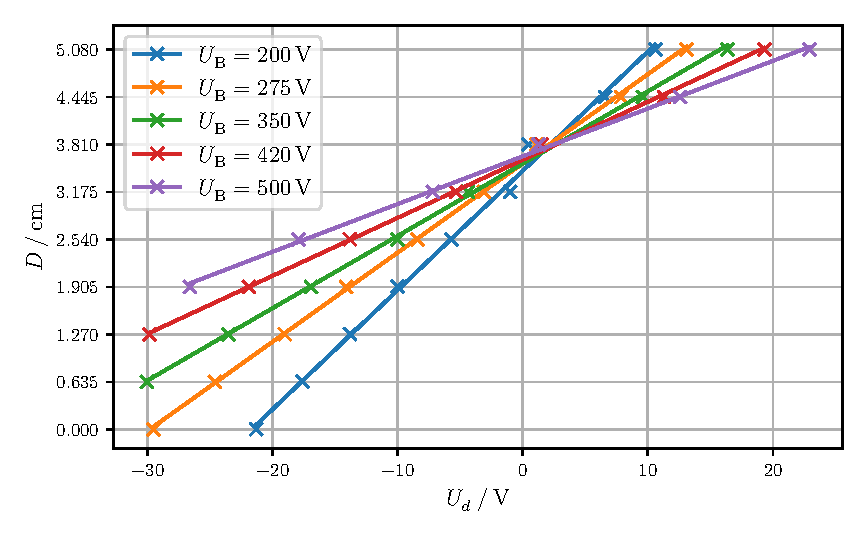
\includegraphics[width=\textwidth]{build/plt/V501_1.pdf}
    \caption{Messwerte und Regressionsgeraden zur Ablenkung im elektrischen Feld.}
    \label{fig:a_501}
\end{figure}

\FloatBarrier
\subsubsection{Bestimmung der Apparaturkonstante}
\label{sec:auswertung:501:apparaturkonstante}

Die soeben gewonnenen Empfindlichkeiten werden nun gegen die jeweilige Beschleunigungsspannung aufgetragen,
um eine weitere Ausgleichsrechnung durchzuführen.
Dazu wird \autoref{eqn:verschiebung} auf beiden Seiten durch $U_\text{d}$ dividiert,
sodass sich
\[ \underbrace{\frac{D}{U_\text{B}}}_{a} = \underbrace{\frac{pL}{2d}}_{c} \cdot \frac{1}{U_\text{B}} \]
ergibt,
wobei $a$ der Steigung der Regressionsgeraden aus dem vorherigen Abschnitt entspricht.
Die Steigung $c$ \textit{dieser} Regressionsgeraden wird zu $\SI{316.26(1125)}{\milli\meter}$ bestimmt.
Werte und Ausgleichgerade sind in \autoref{fig:c_501} dargestellt.

\begin{figure}
   \centering
    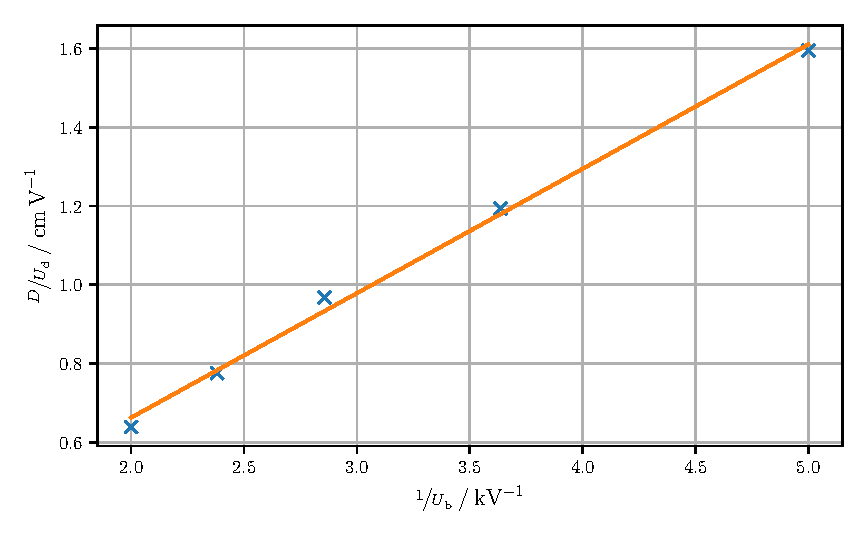
\includegraphics[width=\textwidth]{build/plt/V501_2.pdf}
    \caption{Messwerte und Regressionsgeraden zur Apparaturkonstante.}
    \label{fig:c_501}
\end{figure}

% Da die Werte, aus denen sich die Apparaturkonstante $c$ zusammensetzt,
% bekannt sind, kann auch ein theoretischer Wert angegeben werden.
Die Werte, aus denen sich die Apparaturkonstante $c$ zusammensetzt,
sind bekannt – sie können aus \autoref{fig:abmessungen} entnommen werden.
\begin{align*}
  d &= \SI{0.38}{\centi\meter}
    \tag{Abstand der Y-Ablenkplatten zueinander} \\
  p &= \SI{1.9}{\centi\meter}
    \tag{Länge der Y-Ablenkplatten in Strahlrichtung} \\
  L &= \SI{1.03}{\centi\meter} + \SI{14.3}{\centi\meter} = \SI{15.33}{\centi\meter}
    \tag{Abstand \textbf{Beginn} der Y-Ablenkplatten zum Leuchtschirm} \\
\end{align*}

Daher kann auch ein theoretischer Wert für die Apparaturkonstante angegeben werden:
\[ c_\text{theo} = \frac{pL}{2d} = \SI{357.50}{\milli\meter} \ . \]

% \FloatBarrier
\clearpage
\subsubsection{Frequenz des Sinusgenerators}
\label{sec:auswertung:501:frequenz}

Schließlich soll aus den
wie in \autoref{sec:durchfuehrung:501:frequenz} beschrieben gemessenen
Synchronisationsfrequenzen
die Frequenz der an den Kathodenstrahl-Oszillographen angelegten Sinusspannung
bestimmt werden.
Die \hyperref[eqn:synchronisationsbedingung]{Synchronisationsbedingung} lässt sich auch so beschreiben,
dass die Frequenzen im Verhältnis möglichst einfacher Brüche stehen,
also
\[ \nu_\text{Sä} = k \cdot \nu_\text{We} \qquad k \in \mathbb{Q} \]
gilt.
In \autoref{tab:frequenz_501} sind vier Frequenzen angegeben,
an denen auf dem Leuchtschirm ein stehendes Bild sichtbar ist,
also die Synchronisationsbedingung gilt.
Indem gezählt wird,
wie viele Perioden beziehungsweise wie viele \enquote{Linien} gleichzeitig zu sehen sind,
kann $k$ und somit die Frequenz $\nu_\text{sin}$ der Sinusspannung leicht bestimmt werden.

Entgegen der Beschreibung in \autoref{sec:durchfuehrung:501:frequenz} wurde $k=3$ nicht gemessen,
weil $\nu_\text{Sä}$ nicht niedrig genug eingestellt werden konnte.

\begin{table}
  \centering
  \caption{Sägezahnfrequenzen $\nu_\text{Sä}$, unter denen die Synchronisationsbedingung gilt,
  und Anzahl $k$ der dargestellten Perioden.}
  \label{tab:frequenz_501}
  \begin{tabular}{c S}
  \toprule
  {$k$} &
  {$\nu_\text{Sä} \mathbin{/} \si{\hertz}$} \\
  \midrule
  2            &  25    \\
  1            &  50.01 \\
  \sfrac{1}{2} & 100.02 \\
  \sfrac{1}{3} & 150    \\ %ACHTUNG: 1/3 statt 1/4 wie in unseren Notizen
  \bottomrule
  \end{tabular}
\end{table}

Die Amplitude misst auf dem Leuchtschirm eine halbe Skaleneinheit,
also $\SI{1/8}{inch} = \SI{0.3175}{\centi\meter}$.

Gemäß \autoref{tab:a_501} entspricht das
bei der verwendeten Beschleunigungsspannung
$U_\text{B} = \SI{420}{\volt}$ % nur durch „Reverse engineering“ „bekannt“…
einer Spannungsamplitude von \[ U = \frac{D}{a_{420 V}} = \SI{4.09(6)}{\volt} \ . \]
